\documentclass{article}
\usepackage[utf8]{inputenc}

\title{Feature effect with variale-size bins}
\author{Vasilis Gkolemis}
\date{June 2021}

\usepackage{graphicx}
\usepackage{hyperref}
\usepackage{amsmath}
\usepackage{float}
\graphicspath{ {.} }

\begin{document}

\maketitle

\section{Toy example}

A simple toy example for illustrating the importance of variable-size feature effect. Let's say that the correct feature effect for the feature of interest is (see \ref{im:1}):

\begin{equation} \label{eq:feature-effect}
  f_{\mathtt{ALE}}(x_s) = c +
  \begin{cases}
    10x_s &,  0 \leq x_s < 5 \\
    -10x_s &, 5 \leq x_s < 10 \\
    0 &, 10 \leq x_s < 100 \\
  \end{cases}
\end{equation}
%
where c is a normalizing constant.

\begin{figure}[!h]\label{im:1}
  \centering
  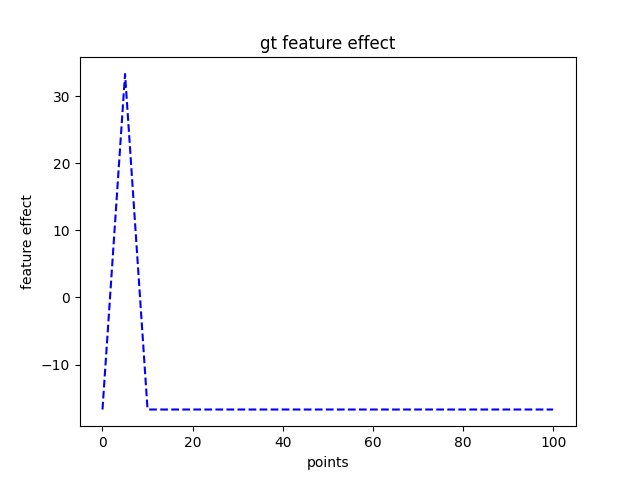
\includegraphics[width=.7\linewidth]{Figure_1.png}
  \caption{Ground-truth feature effect}
\end{figure}


We generate N = 500 datapoints which are distributed in a special way;
\(\frac{500}{3}\) are in \([0,5]\), \(\frac{500}{3}\) in \([5,10]\)
and \(\frac{500}{3}\) in \([10,100]\). The points are more dense in
the first two piecewise linear parts and more narrow later. We also
make the hypothesis that there are correlations with other features,
the local effect computed on each data points gets an added Gaussian
noise:

\begin{equation} \label{eq:data-effect}
  \frac{\partial f}{ \partial x_s} (x_s) = \epsilon +
  \begin{cases}
    10 &,  0 \leq x_s < 5 \\
    -10 &, 5 \leq x_s < 10 \\
    0 &, 10 \leq x_s < 100 \\
  \end{cases}
\end{equation}

where \(\epsilon \sim \mathcal{N}(0, 2)\). See the local effect of
each data point in figure \ref{im:2}.


\begin{figure}[!h]\label{im:2}
\centering
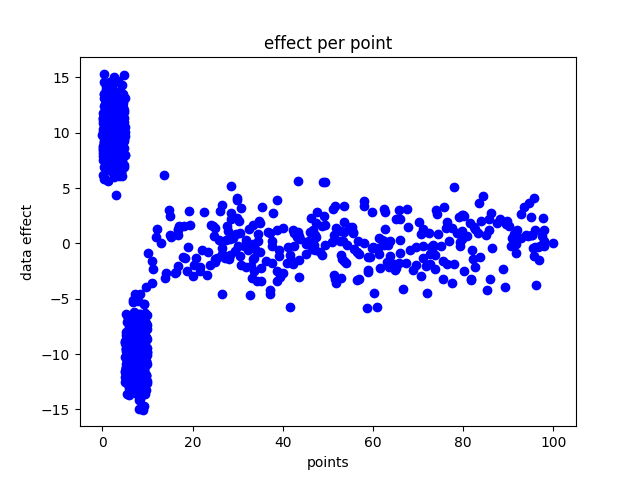
\includegraphics[width=0.7\linewidth]{Figure_2.png}
\caption{Local effect per point}
\end{figure}

The example is created to highlight the importance of variable bins;
there are two very strong effects in areas \([0,5]\), \([5,10]\), and
then the effect is zero. Ideally, we would like to create only three
bins of different-size, i.e. \([0,5]\), \([5,10]\), \([10,100]\).


\section{Fixed-size}

With fixed-size bins, there are two solutions; If we create large bins
we miss the first two high-resolution effects at the begining (see
fig.\ref{im:fixed-10}). If we create small bins, we capture the
effects at the beginning, but we split effect of \([10,100]\) in many
bins leading to noisy artifacts (see fig \ref{im:fixed-100},
\ref{im:fixed-1000}).

\begin{figure}[!h]
\centering
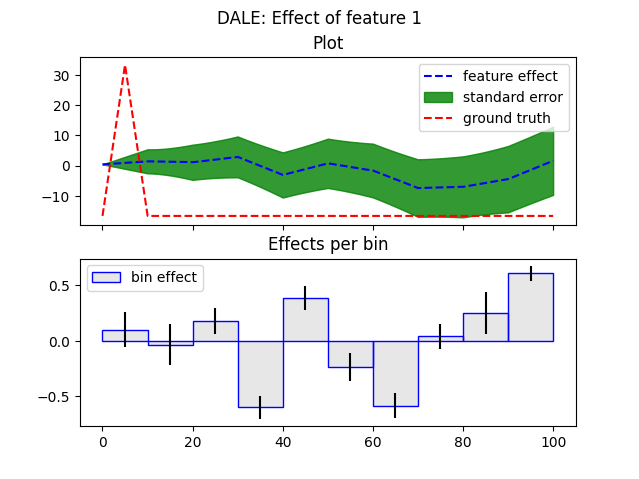
\includegraphics[width=0.9\linewidth]{Figure_dale_fixed_10.png}
\caption{DALE fixed-size with 10 bins}
\label{im:fixed-10}
\end{figure}

\begin{figure}[!h]
\centering
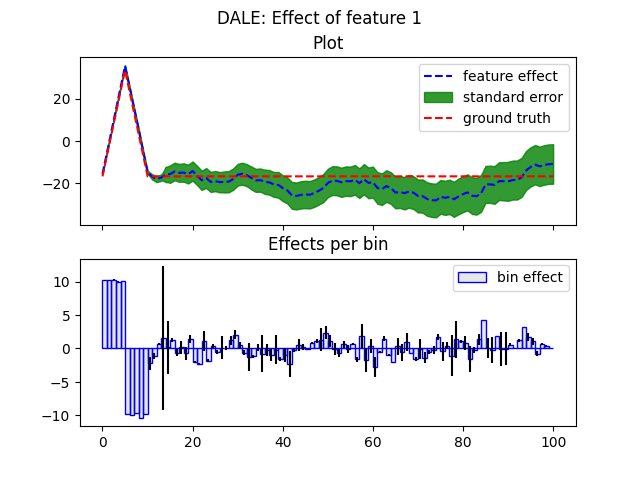
\includegraphics[width=0.9\linewidth]{Figure_dale_fixed_100.png}
\caption{DALE fixed-size with 100 bins}
\label{im:fixed-100}
\end{figure}

\begin{figure}[!h]
\centering
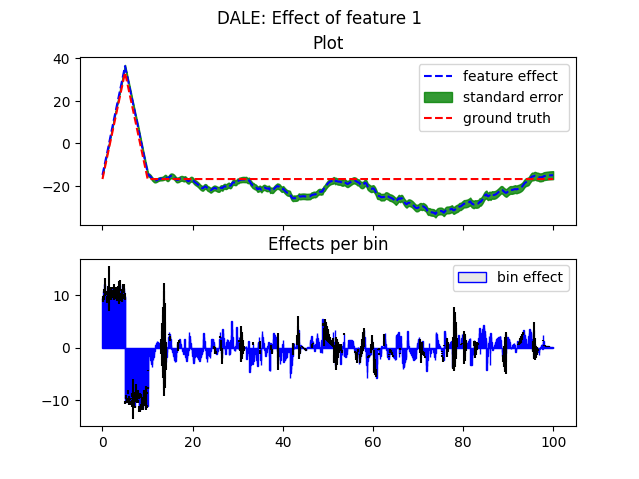
\includegraphics[width=0.9\linewidth]{Figure_dale_fixed_1000.png}
\caption{DALE fixed-size with 1000 bins}
\label{im:fixed-1000}
\end{figure}


\section{Variable-size}

With variable-size we can find the optimal bins, given that there is
enough resolution i.e. the maximum number of bins is large enough to
enable creating small bins in the beginning. For example, with maximum
number of bins equal to 10 (see figure \ref{im:var-10}), it is
impossible to capture the effect in the beginning. But with maximum
number of bins \(\geq 20\) (see \ref{im:var-20} \ref{im:var-100}), the
bins are created (almost) perfectly. We also observe that the actual
number of the hyperparamer maximum number of bins is not important;
all values \(\geq 20\) give robust results. Finally, we confirm that
with create the 'correct' bins, we create perfect feature effect
(almost identical with the ground-truth).

\begin{figure}[!h]
\centering
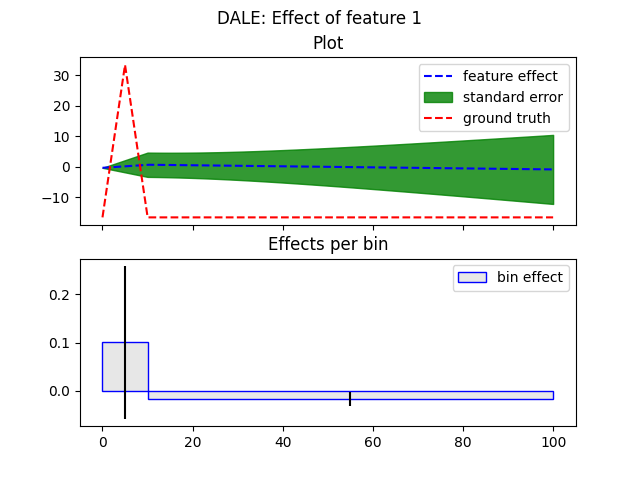
\includegraphics[width=0.9\linewidth]{Figure_dale_var_10.png}
\caption{DALE variable-size with 10 bins}
\label{im:var-10}
\end{figure}

\begin{figure}[!h]
\centering
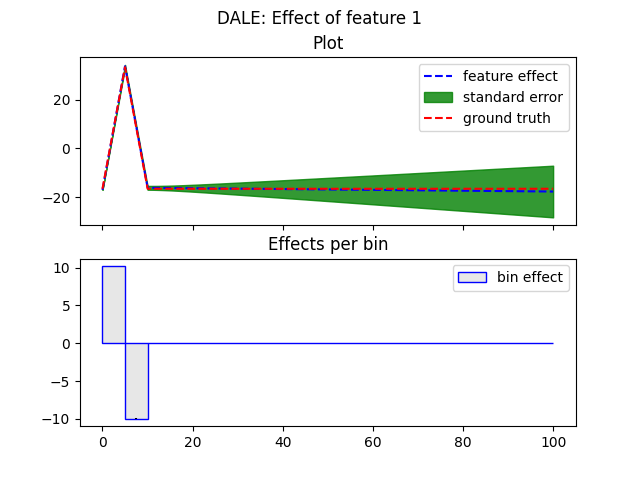
\includegraphics[width=0.9\linewidth]{Figure_dale_var_20.png}
\caption{DALE variable-size with 20 bins}
\label{im:var-20}
\end{figure}

\begin{figure}[!h]
\centering
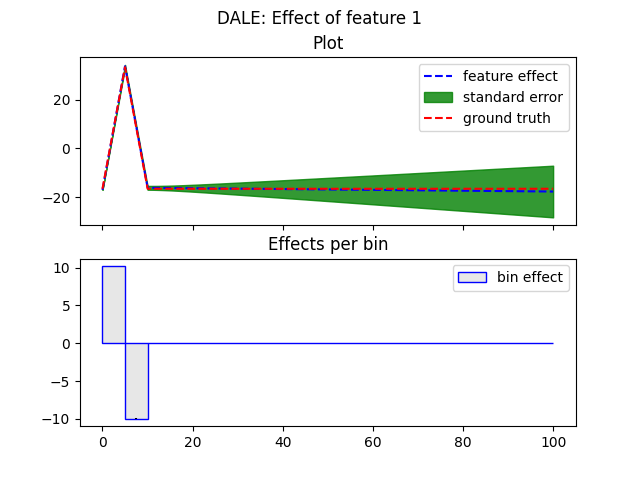
\includegraphics[width=0.9\linewidth]{Figure_dale_var_100.png}
\caption{DALE variable-size with 100 bins}
\label{im:var-100}
\end{figure}


\section{Comparing fixed-size with Variable-size}

We evaluate fixed-size and variable-size with two metrics; Loss and
MSE. Loss is the sum of the standard error of each bin and MSE is the
Mean squared error between the obtained feature effect plot and the
ground-truth. Our goal is to choose the plot with minimum sum of
standard errors (loss) as the best feature effect
estimation. Therefore, we want to check whether minimising the loss is
a good criterion for getting the plot with the smallest MSE. We set a
threshold of mimimum 10 points per bin for ensuring robust standard
error estimations. Therefore we cannot evaluate the loss in cases of
large number of fixed-size bins.

For the loss, in figure \ref{im:loss} we obsere that:

\begin{itemize}
\item for fixed size, the standard error is not a good indicator for
  choosing the correct number of bins. Firstly, we cannot evaluate it
  for large number of bins, since there are not enough points inside
  all bins. Secondly, since the variance inside the bins is big,
  standard error is dominated by the number of samples.
\item for variable size, the sum of standard errors is a valid
  indicator indicator. When loss is minimized (K=20, 40, 60) the MSE
  is also minimized.
\end{itemize}

\begin{figure}[h]
\centering
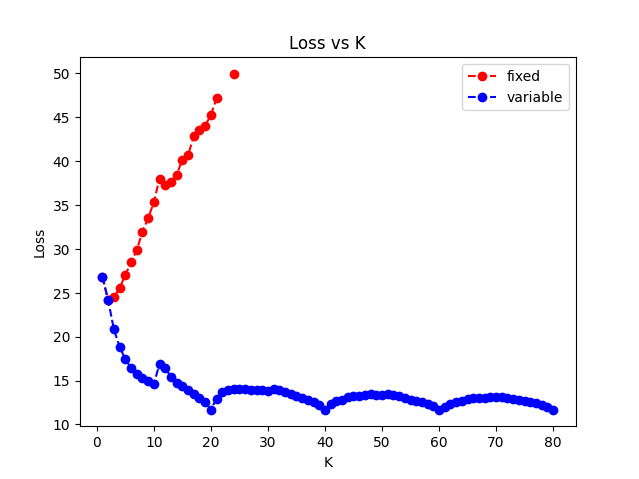
\includegraphics[width=0.9\linewidth]{Figure_7.png}
\caption{Loss vs number of bins (means number of bins when fixed size, and maximum number of bins when variable size)}
\label{im:loss}
\end{figure}


For the MSE, in figure \ref{im:mse}, we obsere that:

\begin{itemize}
\item for fixed-size, the MSE is smaller for larger number of bins (makes sense)
\item for variable-size, the MSE is smaller for larger maximum number of bins (makes sense)
\item the variable-size creates in general more accurate feature effect plots
\item as the maximum number of bins grows larger we get more robust
  feature effect plots. For example, K=21 leads to large MSE, whereas K=20 is almost optimal. In contrast, K=71 is very close to K=70 which is also almost optimal. In general, for K>50 the result is close to perfect independently of the exact value of K.
\end{itemize}

\begin{figure}[h]
\centering
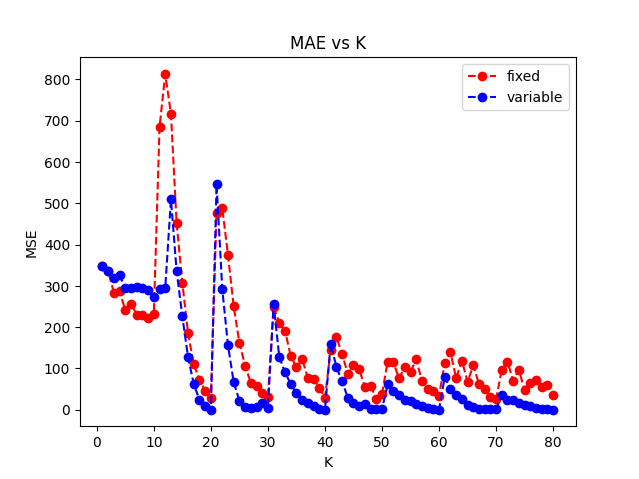
\includegraphics[width=0.9\linewidth]{Figure_9.png}
\caption{MSE vs number of bins (means number of bins when fixed size, and maximum number of bins when variable size)}
\label{im:mse}
\end{figure}




\section{Best solutions based on standard error}

In figure \ref{im:best-fixed} we see the best fixed-size feature
effect plot based on loss and in figure \ref{im:best-var} the best variable-size based on the same criterion.

\begin{figure}[h]
\centering
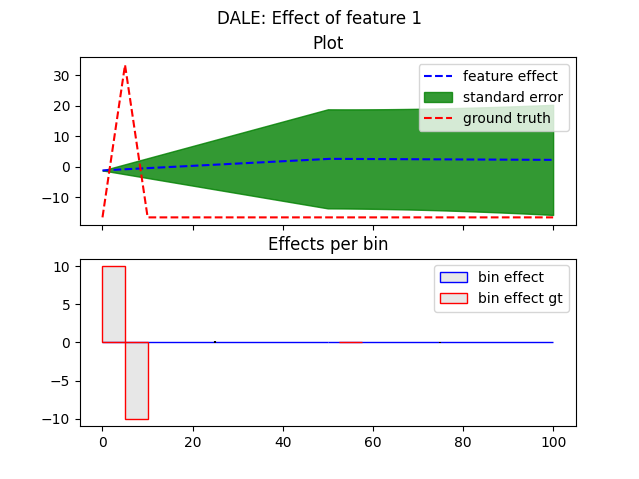
\includegraphics[width=0.9\linewidth]{Figure_10.png}
\caption{Best solution, based on standard error, for fixed-size bins is the creation of 2 bins}
\label{im:best-fixed}
\end{figure}

\begin{figure}[h]
\centering
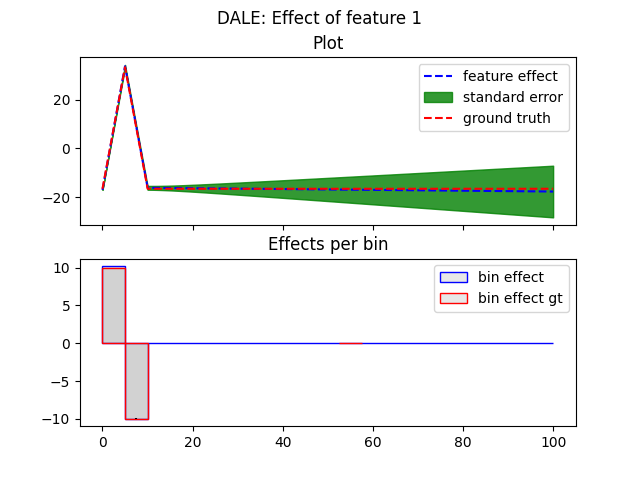
\includegraphics[width=0.9\linewidth]{Figure_11.png}
\caption{Best solution based on standard error for variable-size bins; it creates the 3 correct bins, with maximum number of bins equal to 80.}
\label{im:best-var}
\end{figure}

\section{Conclusion}

It is easy to show that it is important to create plots of
variable-size bins. Sum of standard errors can be an indicator for
choosing the correct plot, but it is not very robust. When the
clusters are not very clear, it tends to choose bigger bins (sometimes
even allocating all points in a single bin). I am still searching for
alternative clustering criteria.


\end{document}
